\documentclass[11pt,a4paper]{article}

% =========================================================================
% PACKAGES
% =========================================================================
\usepackage[utf8]{inputenc}
\usepackage[margin=1.8cm,top=1.8cm,bottom=1.8cm]{geometry}
\usepackage{graphicx}
\usepackage{booktabs}
\usepackage{tabularx}
\usepackage{titlesec}
\usepackage{fancyhdr}
\usepackage{subcaption}
\usepackage{float}
\usepackage{hyperref}

% Clean black and white hyperref setup
\hypersetup{
    colorlinks=true,
    linkcolor=black,
    citecolor=black,
    urlcolor=black
}

% Clean, formal serif section titles (White Theme - No color bars)
\titleformat{\section}
  {\normalfont\Large\bfseries}{\thesection}{1em}{}[{\titlerule[0.8pt]}]

\titleformat{\subsection}
  {\normalfont\large\bfseries}{\thesubsection}{1em}{}

\setlength{\parindent}{0pt}
\setlength{\parskip}{6pt}

% Header & Footer
\pagestyle{fancy}
\fancyhf{}
\lhead{\footnotesize IIITDM Kurnool --- Department of ECE | EPM Laboratory}
\rhead{\footnotesize Divyansh Rawat (124EC0030)}
\cfoot{\thepage}
\renewcommand{\headrulewidth}{0.4pt}
\renewcommand{\footrulewidth}{0.4pt}

% =========================================================================
\begin{document}

% =========================================================================
% PAGE 1: OFFICIAL IIITDM KURNOOL CERTIFICATE & COVER PAGE
% =========================================================================
\thispagestyle{empty}

\begin{center}
    
\includegraphics[width=2.8cm]{iiitdm_logo.png}\\[8pt]
    {\Large \textbf{INDIAN INSTITUTE OF INFORMATION TECHNOLOGY}}\\[2pt]
    {\Large \textbf{DESIGN AND MANUFACTURING KURNOOL}}\\[4pt]
    {\small (An Institute of National Importance under Ministry of Education, Govt. of India)}\\[2pt]
    {\footnotesize Jagannathagattu, Dinnedevarapadu, Kurnool -- 518008, Andhra Pradesh}\\[20pt]
\end{center}

\begin{flushright}
    \textbf{Reg. No. : 124EC0030}
\end{flushright}

\vspace{4mm}

\begin{center}
    \fbox{\Large \textbf{\quad CERTIFICATE \quad}}
\end{center}

\vspace{6mm}

\begin{center}
    \normalsize
    Certified that this is the bonafide record of practical work done\\[14pt]
    by \textbf{Mr. Divyansh Rawat (Reg. No: 124EC0030)}\\[14pt]
    of the \textbf{Department of Electronics and Communication Engineering}\\[14pt]
    in the \textbf{Electronic Prototyping and Manufacturing (EPM) Laboratory}\\[14pt]
    for the End Semester Practical Examination on\\[4pt]
    \textbf{Dual Inductance-Sensitive Tone Demonstrator --- Layout Variant A ($90 \times 70$\,mm)}\\[14pt]
    during the academic year 2026 -- 2027.\\[14pt]
    \textbf{Course Faculty:} Dr. Eswaramoorthy K V
\end{center}

\vspace{6mm}

\begin{table}[H]
\centering
\small
\renewcommand{\arraystretch}{1.3}
\begin{tabular}{|l|l|}
\hline
\textbf{Student Name:} & Divyansh Rawat (Roll No: 124EC0030) \\ \hline
\textbf{Course Faculty / Examiner:} & Dr. Eswaramoorthy K V \\ \hline
\textbf{Date of Examination:} & 10-11-2026 \\ \hline
\textbf{Examination Pattern:} & Layout Variant A ($90 \times 70$\,mm Double-Layer PCB) \\ \hline
\textbf{Verification Status:} & 0 ERC Errors, 0 DRC Violations (100\% Netlist Parity) \\ \hline
\end{tabular}
\end{table}

\vfill

% Signatures positioned exactly as in IIITDM template
\noindent
\begin{tabularx}{\textwidth}{X r}
\textbf{Signature of Head of the Department} & \textbf{Signature of Faculty} \\[25pt]
 & \textbf{Dr. Eswaramoorthy K V} \\[4pt]
 & \textit{Associate Professor, Dept. of ECE} \\[6pt]
Date: \rule{4cm}{0.4pt} & Date: \rule{4cm}{0.4pt} \\
\end{tabularx}

\clearpage

% =========================================================================
% PAGE 2: ITEM 1 - CIRCUIT DIAGRAM (REFERENCE SPECIFICATION)
% =========================================================================
\section{Circuit Diagram (Reference Circuit Specification)}

\textbf{Source Reference:} 555-Timer-Circuits.com Metal Detector / Dual Inductance-Sensitive Tone Generator.

\textbf{Principle of Operation:} The circuit operates as an astable multivibrator utilizing the classic NE555 timer IC. The oscillation frequency is governed by the inductive reactance of the 10\,mH external choke ($L_1$) interacting with timing capacitors $C_3, C_4$ ($2.2\,\mu\text{F}$) and feedback timing resistor $R_2$ ($47\,\text{k}\Omega$). When a metallic or ferromagnetic object approaches the external inductor, the effective inductance shifts, modulating the astable timing cycle and producing an audible frequency change through the $8\,\Omega$ loudspeaker coupled via capacitor $C_5$ ($10\,\mu\text{F}$).

\vspace{3mm}

\begin{figure}[H]
    \centering
    \begin{subfigure}[b]{0.46\textwidth}
        \centering
        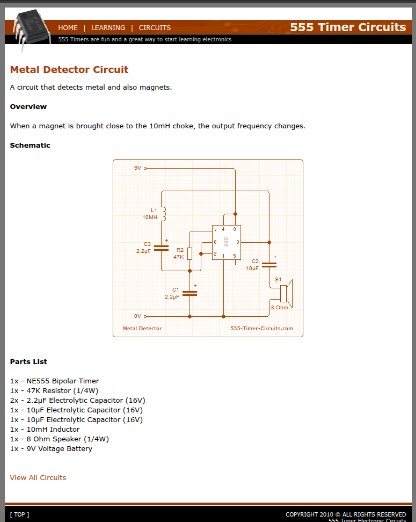
\includegraphics[width=\textwidth]{screenshots/01_Reference_Website_Spec.png}
        \caption{Source website specification and parts list.}
    \end{subfigure}
    \hfill
    \begin{subfigure}[b]{0.51\textwidth}
        \centering
        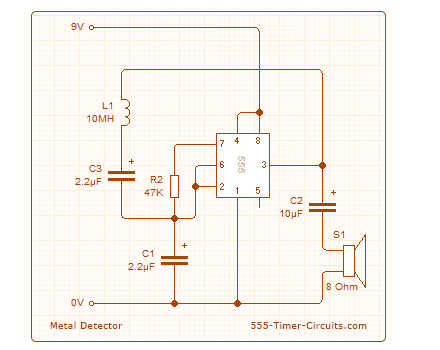
\includegraphics[width=\textwidth]{screenshots/01_Reference_Circuit_Diagram.png}
        \caption{Enlarged reference schematic diagram.}
    \end{subfigure}
    \caption{Source reference documentation from 555-Timer-Circuits.com.}
\end{figure}

\clearpage

% =========================================================================
% PAGE 3: ITEM 2 - SCHEMATIC DIAGRAM
% =========================================================================
\section{Schematic Diagram (KiCad Schematic Editor)}

Live interactive KiCad Schematic Editor capture showing the complete dual-channel 555 oscillator design. The schematic is modularly partitioned into four functional sections:
\begin{enumerate}
    \item \textbf{Power Supply Conditioning (9\,V DC):} Bulk reservoir filtering ($C_1 = 100\,\mu\text{F}$), high-frequency decoupling ($C_2 = 100\,\text{nF}$), power status LED indicator ($D_1$ with ballast resistor $R_1 = 1\,\text{k}\Omega$), and test points (\texttt{TP\_9V}, \texttt{TP\_GND}).
    \item \textbf{Channel A 555 Oscillator:} Timer IC $U_1$, astable loop ($R_2, C_3, C_4$), inductor connector $J_2$ (\texttt{L\_A}), local $100\,\text{nF}$ bypass capacitor $C_6$, speaker coupling ($C_5, C_7$), and output header $J_3$ (\texttt{SPK\_A}).
    \item \textbf{Channel B 555 Oscillator:} Symmetrical timer IC $U_2$, astable loop ($R_3, C_8, C_9$), inductor connector $J_4$ (\texttt{L\_B}), local $100\,\text{nF}$ bypass capacitor $C_{11}$, speaker coupling ($C_{10}, C_{12}$), and output header $J_5$ (\texttt{SPK\_B}).
    \item \textbf{Mechanical Chassis Mounting:} Four isolated non-plated M3 chassis mounting holes ($H_1$--$H_4$) located at the board corners.
\end{enumerate}

\vspace{2mm}

\begin{figure}[H]
    \centering
    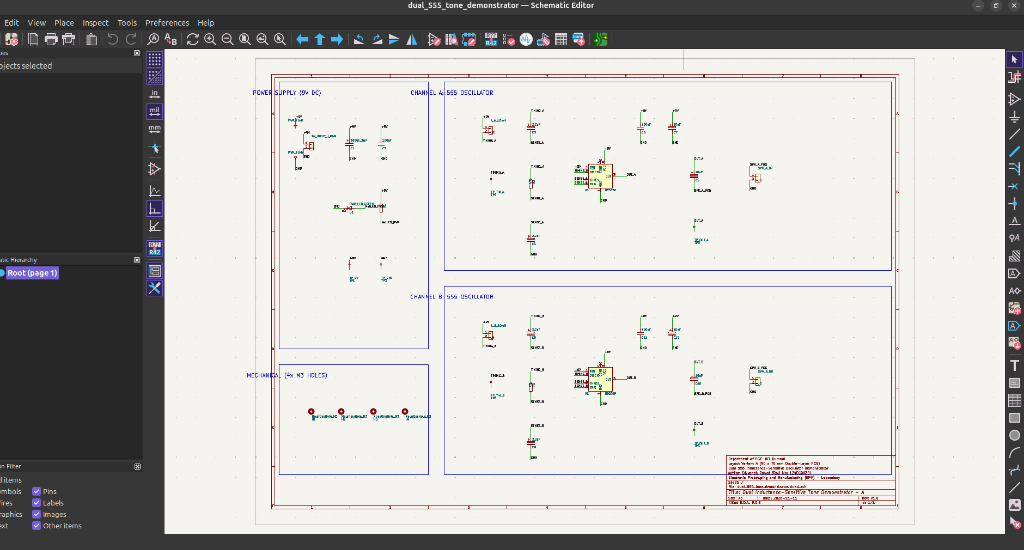
\includegraphics[width=0.98\textwidth]{screenshots/02_Schematic_Diagram_KiCad.png}
    \caption{Full schematic sheet captured in KiCad Schematic Editor (Sheet size: A3, with formal title block).}
\end{figure}

\vspace{-2mm}

\begin{table}[H]
\centering
\small
\renewcommand{\arraystretch}{1.2}
\begin{tabular}{|l|p{4.2cm}|l|p{4.2cm}|}
\hline
\textbf{Sheet Size / Frame:} & A3 ($420 \times 297$\,mm, Standard Frame) & \textbf{Hierarchy:} & Flat Single Sheet (Root /) \\ \hline
\textbf{Oscillator Channels:} & 2 Symmetrical 555 Astable Circuits & \textbf{Decoupling Capacitors:} & 100\,nF Ceramic per IC (Pin 8 to GND) \\ \hline
\textbf{ERC Verification:} & 0 Errors, 0 Warnings (PASSED) & \textbf{Course Faculty:} & Dr. Eswaramoorthy K V \\ \hline
\end{tabular}
\end{table}

\clearpage

% =========================================================================
% PAGE 4: ITEM 3 - COMPOSITE PCB LAYOUT
% =========================================================================
\section{Composite PCB Layout (KiCad PCB Editor)}

Live interactive PCB Editor screenshot showing double-sided routing (\texttt{F.Cu} red, \texttt{B.Cu} blue), continuous solid ground planes with thermal relief spokes, component placements, and \texttt{Edge.Cuts} boundary.

\textbf{Placement Constraints Satisfied:}
\begin{itemize}
    \item \textbf{Left Edge:} DC power supply terminal block ($J_1$) located centrally on the left border.
    \item \textbf{Lower Edge:} External inductor input connectors $J_2$ (\texttt{L\_A}) and $J_4$ (\texttt{L\_B}) aligned along the bottom edge.
    \item \textbf{Upper Edge:} External speaker output connectors $J_3$ (\texttt{SPK\_A}) and $J_5$ (\texttt{SPK\_B}) aligned along the top edge.
    \item \textbf{Short Timing Loops:} Timing capacitors ($C_3, C_4$ and $C_8, C_9$) and resistors ($R_2, R_3$) positioned adjacent to pins 2, 6, and 7 of each 555 IC.
    \item \textbf{Mounting Holes:} 4x M3 mounting holes with 6.0\,mm keepout zones positioned at $(x=\pm 5\,\text{mm}, y=\pm 5\,\text{mm})$ from corners.
\end{itemize}

\vspace{2mm}

\begin{figure}[H]
    \centering
    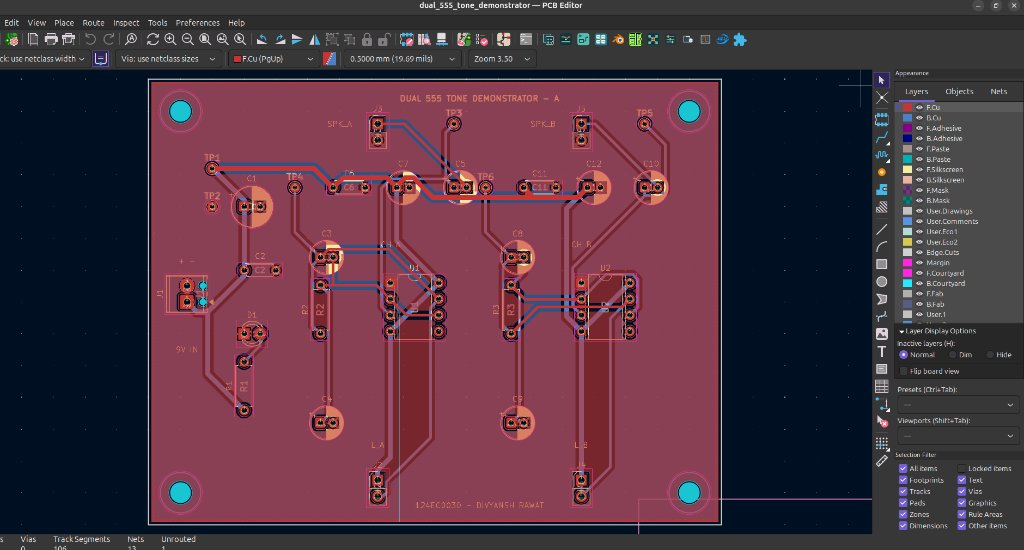
\includegraphics[width=0.98\textwidth]{screenshots/03_Composite_PCB_Layout.jpg}
    \caption{Interactive layout view in KiCad PCB Editor displaying double-sided routing and polygon copper zones.}
\end{figure}

\vspace{-2mm}

\begin{table}[H]
\centering
\small
\renewcommand{\arraystretch}{1.2}
\begin{tabular}{|l|p{4.2cm}|l|p{4.2cm}|}
\hline
\textbf{Board Dimensions:} & $90.00 \times 70.00$\,mm (Rectangular) & \textbf{Layer Stackup:} & 2 Copper Layers (F.Cu \& B.Cu, 1.6\,mm FR4) \\ \hline
\textbf{Component Count:} & 23 Through-Hole Components & \textbf{Routing Completion:} & 49 / 49 Nets (100\% Routed, 0 Unrouted) \\ \hline
\textbf{Mounting Holes:} & 4x M3 (3.2\,mm NPTH, 6.0\,mm Keepout) & \textbf{Test Points:} & 6 THT Diagnostic Pads (TP1--TP6) \\ \hline
\end{tabular}
\end{table}

\clearpage

% =========================================================================
% PAGE 5: ITEM 4 - FRONT COPPER LAYER (F.Cu)
% =========================================================================
\section{Front Copper Layer (F.Cu)}

Live KiCad PCB Editor layer inspection view showing top-layer copper routing (\texttt{F.Cu}) with all inactive layers hidden. Features 0.50\,mm wide power distribution tracks (+9\,V DC rail) and 0.30\,mm signal tracks. All trace corners utilize 45-degree mitered chamfers (0.60\,mm setback) to eliminate 90-degree acid traps during chemical board etching.

\vspace{3mm}

\begin{figure}[H]
    \centering
    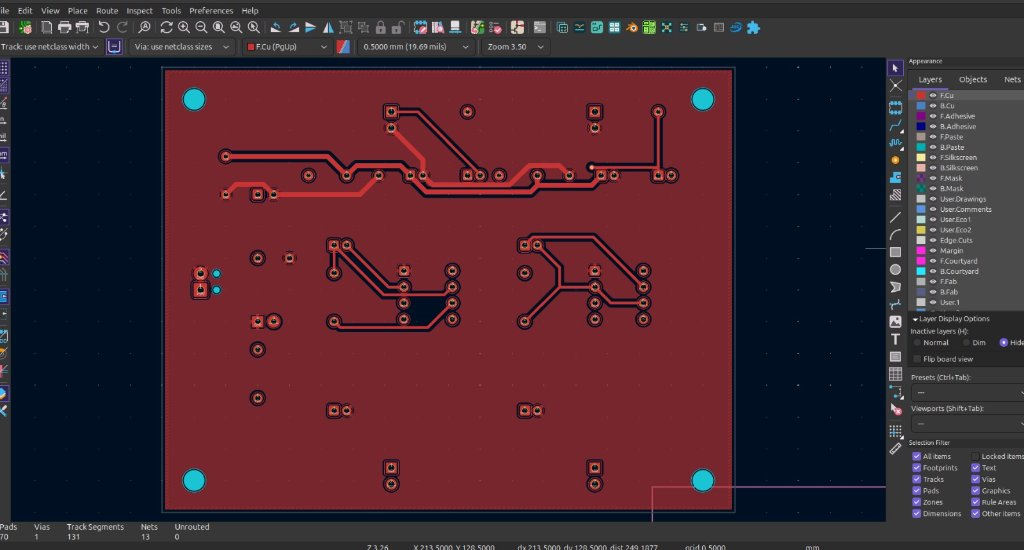
\includegraphics[width=0.98\textwidth]{screenshots/04_Front_Copper_F_Cu.jpg}
    \caption{Front copper layer (\texttt{F.Cu}) routing captured with Inactive Layers set to Hide in KiCad.}
\end{figure}

\vspace{-2mm}

\begin{table}[H]
\centering
\small
\renewcommand{\arraystretch}{1.2}
\begin{tabular}{|l|p{4.2cm}|l|p{4.2cm}|}
\hline
\textbf{Layer Identifier:} & \texttt{F.Cu} (Top Copper, Red) & \textbf{Finished Copper:} & 35\,$\mu$m (1.0\,oz/ft$^2$) \\ \hline
\textbf{Power Track Width:} & 0.50\,mm (19.69\,mils, Net \texttt{/+9V}) & \textbf{Signal Track Width:} & 0.30\,mm (11.81\,mils) \\ \hline
\textbf{Minimum Clearance:} & 0.25\,mm (9.84\,mils, Design Rule) & \textbf{Corner Mitering:} & 45$^\circ$ Diagonal Setbacks (No 90$^\circ$ Bends) \\ \hline
\end{tabular}
\end{table}

\clearpage

% =========================================================================
% PAGE 6: ITEM 5 - BACK COPPER LAYER (B.Cu)
% =========================================================================
\section{Back Copper Layer (B.Cu)}

Live KiCad PCB Editor layer inspection view showing bottom-layer copper routing (\texttt{B.Cu}) with all inactive layers hidden. Provides an expansive, low-impedance ground return plane with thermal relief spoke connections to through-hole GND pads. Interconnects Channel A and Channel B oscillator timing sub-circuits while preserving return current continuity.

\vspace{3mm}

\begin{figure}[H]
    \centering
    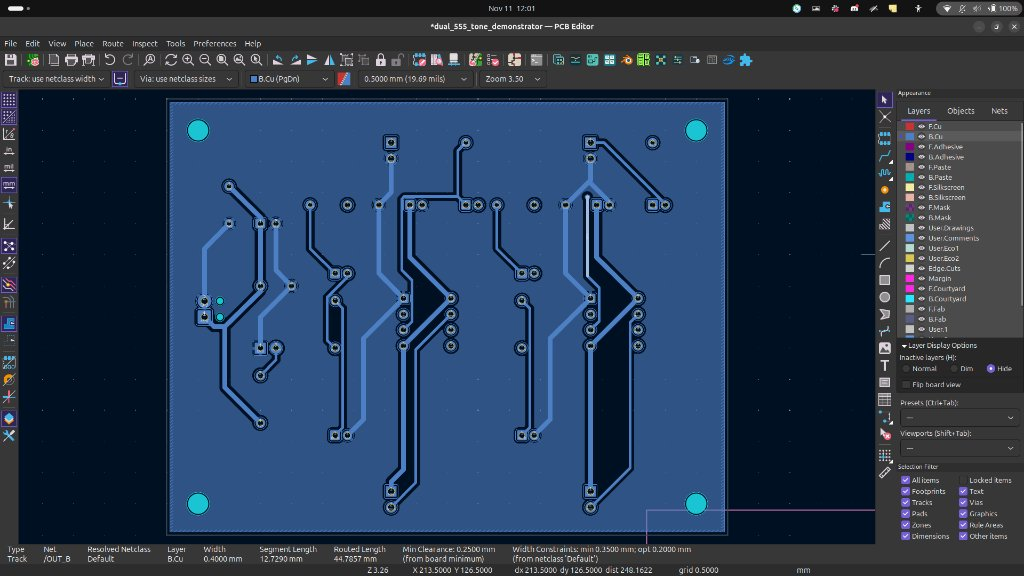
\includegraphics[width=0.98\textwidth]{screenshots/05_Back_Copper_B_Cu.jpg}
    \caption{Back copper layer (\texttt{B.Cu}) routing captured with Inactive Layers set to Hide in KiCad.}
\end{figure}

\vspace{-2mm}

\begin{table}[H]
\centering
\small
\renewcommand{\arraystretch}{1.2}
\begin{tabular}{|l|p{4.2cm}|l|p{4.2cm}|}
\hline
\textbf{Layer Identifier:} & \texttt{B.Cu} (Bottom Copper, Blue) & \textbf{Finished Copper:} & 35\,$\mu$m (1.0\,oz/ft$^2$) \\ \hline
\textbf{Ground Plane Pour:} & Solid Continuous Zone (Net \texttt{/GND}) & \textbf{Thermal Spokes:} & 4 Spokes (0.50\,mm width, 0.35\,mm gap) \\ \hline
\textbf{Isolated Copper:} & 0 Unconnected Copper Islands & \textbf{Corner Mitering:} & 45$^\circ$ Diagonal Setbacks (No 90$^\circ$ Bends) \\ \hline
\end{tabular}
\end{table}

\clearpage

% =========================================================================
% PAGE 7: ITEM 6 - SILKSCREEN LAYER (F.SilkS)
% =========================================================================
\section{Silkscreen Layer (F.SilkS)}

Live KiCad PCB Editor layer inspection view showing the front silkscreen legend (\texttt{F.SilkS}) with all inactive layers hidden. Contains unambiguous component outlines, reference designators ($U_1$--$U_2$, $R_1$--$R_3$, $C_1$--$C_{12}$, $D_1$, $J_1$--$J_5$, $\text{TP}_1$--$\text{TP}_6$), polarity indicators (+/$-$ for 9\,V IN, pin 1 notches for DIP-8 ICs, and electrolytic capacitor positive markings), connector labels (\texttt{9V IN}, \texttt{L\_A}, \texttt{L\_B}, \texttt{SPK\_A}, \texttt{SPK\_B}), and student roll number identification.

\vspace{3mm}

\begin{figure}[H]
    \centering
    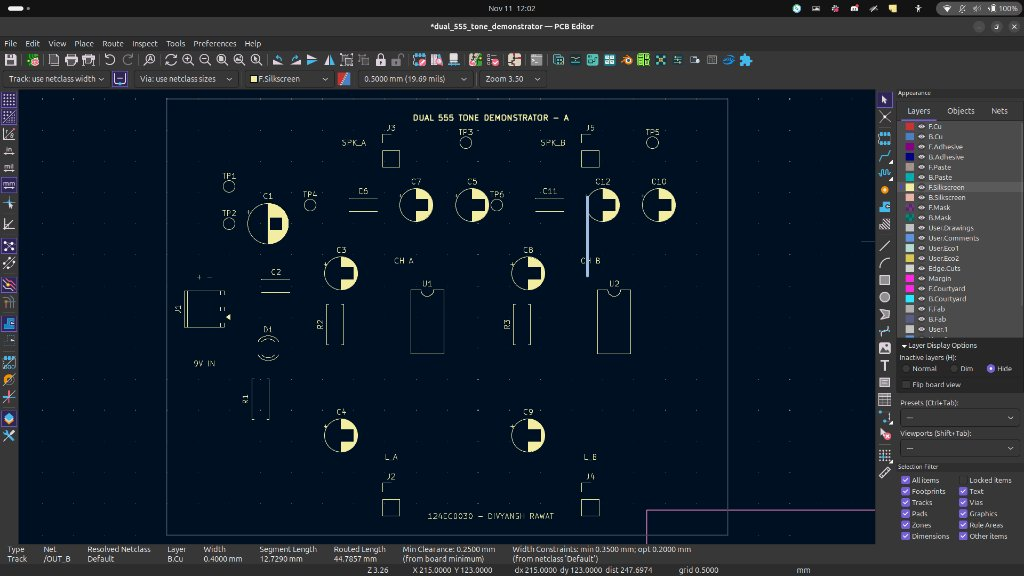
\includegraphics[width=0.98\textwidth]{screenshots/06_Silkscreen_F_SilkS.jpg}
    \caption{Front silkscreen layer (\texttt{F.SilkS}) legend captured with Inactive Layers set to Hide in KiCad.}
\end{figure}

\vspace{-2mm}

\begin{table}[H]
\centering
\small
\renewcommand{\arraystretch}{1.2}
\begin{tabular}{|l|p{4.2cm}|l|p{4.2cm}|}
\hline
\textbf{Layer Identifier:} & \texttt{F.SilkS} (Front Silkscreen, White) & \textbf{Color Contrast:} & High-Opacity White on Green Soldermask \\ \hline
\textbf{Text Height / Width:} & 1.0\,mm / 1.5\,mm (0.15\,mm line thickness) & \textbf{Polarity Marking:} & 9V IN (+/$-$), L A/B, SPK A/B, C1--C12 (+) \\ \hline
\textbf{Student Attribution:} & \texttt{124EC0030 --- DIVYANSH RAWAT} & \textbf{Board Title:} & \texttt{DUAL 555 TONE DEMONSTRATOR - A} \\ \hline
\end{tabular}
\end{table}

\clearpage

% =========================================================================
% PAGE 8: ITEM 7 - SOLDER MASK LAYER (F.Mask & B.Mask)
% =========================================================================
\section{Solder Mask Layer (F.Mask \& B.Mask)}

Live KiCad PCB Editor layer inspection views showing solder mask apertures with inactive layers hidden. Top apertures (\texttt{F.Mask}, purple) and bottom apertures (\texttt{B.Mask}, teal) provide 0.10\,mm radial clearance around all through-hole component pads, test points, terminal blocks, and mounting holes to prevent solder bridging during hand assembly.

\vspace{3mm}

\begin{figure}[H]
    \centering
    \begin{subfigure}[b]{0.48\textwidth}
        \centering
        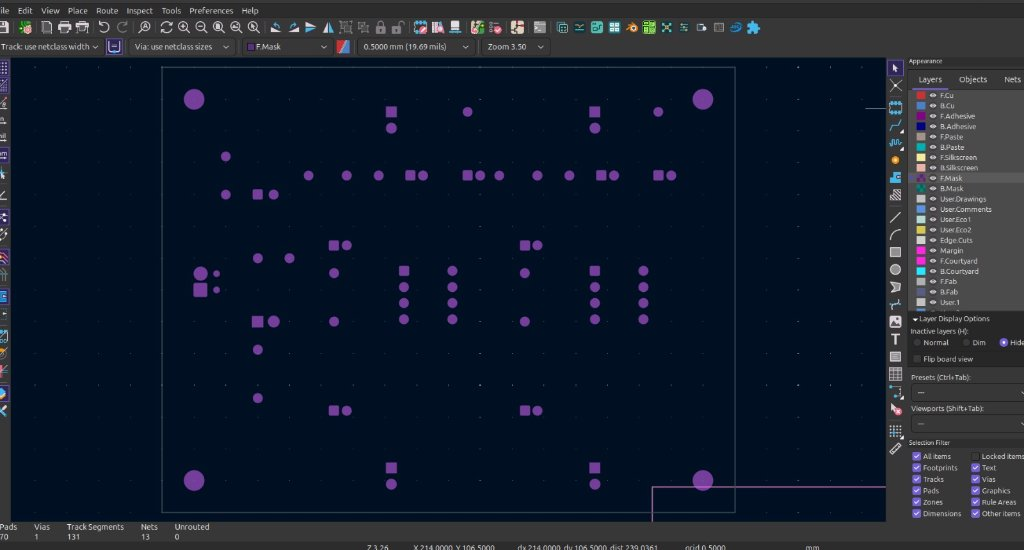
\includegraphics[width=\textwidth]{screenshots/07_Solder_Mask_Front_F_Mask.jpg}
        \caption{Front Solder Mask Apertures (\texttt{F.Mask} --- Component Side).}
    \end{subfigure}
    \hfill
    \begin{subfigure}[b]{0.48\textwidth}
        \centering
        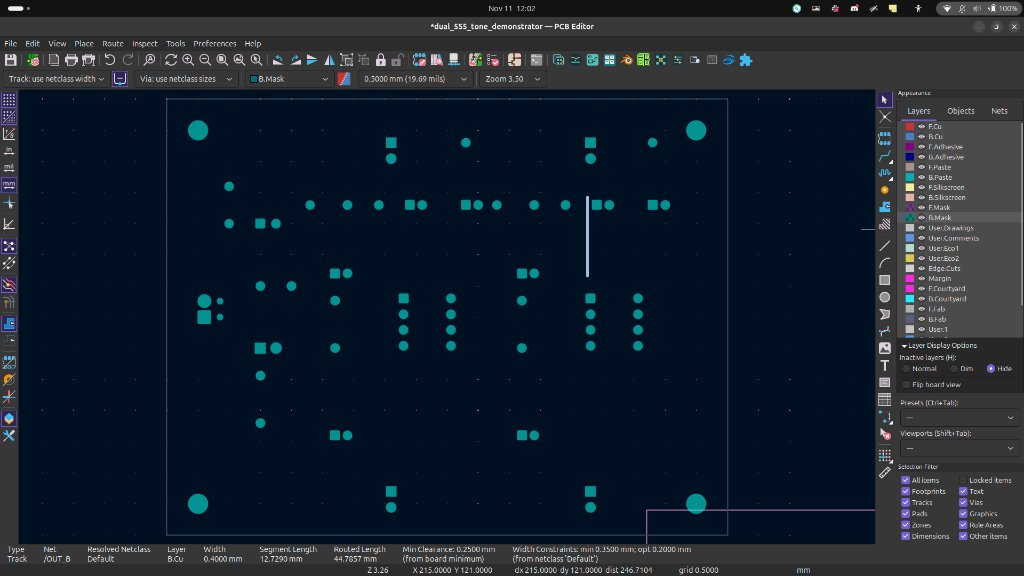
\includegraphics[width=\textwidth]{screenshots/07_Solder_Mask_Back_B_Mask.jpg}
        \caption{Back Solder Mask Apertures (\texttt{B.Mask} --- Solder Side).}
    \end{subfigure}
    \caption{Solder mask apertures captured in KiCad PCB Editor with Inactive Layers set to Hide.}
\end{figure}

\vspace{-2mm}

\begin{table}[H]
\centering
\small
\renewcommand{\arraystretch}{1.2}
\begin{tabular}{|l|p{4.2cm}|l|p{4.2cm}|}
\hline
\textbf{Radial Mask Clearance:} & 0.10\,mm (Board Design Rules) & \textbf{Minimum Solder Dam:} & 0.10\,mm Web Between Adjacent Pads \\ \hline
\textbf{Pad Aperture Coverage:} & All 70 THT Component \& Connector Pads & \textbf{Solder Mask Material:} & Liquid Photoimageable (LPI) Green \\ \hline
\end{tabular}
\end{table}

\clearpage

% =========================================================================
% PAGE 9: ITEM 8 - ELECTRICAL RULES CHECK (ERC) SCREENSHOT
% =========================================================================
\section{Screenshot of Electrical Rules Check (ERC)}

Live KiCad Schematic Editor Electrical Rules Checker dialog showing \textbf{0 Errors, 0 Warnings, and 0 Violations}. Confirms that all pin electrical types, power flag drivers, net connectivity, and label references strictly comply with design rules.

\vspace{3mm}

\begin{figure}[H]
    \centering
    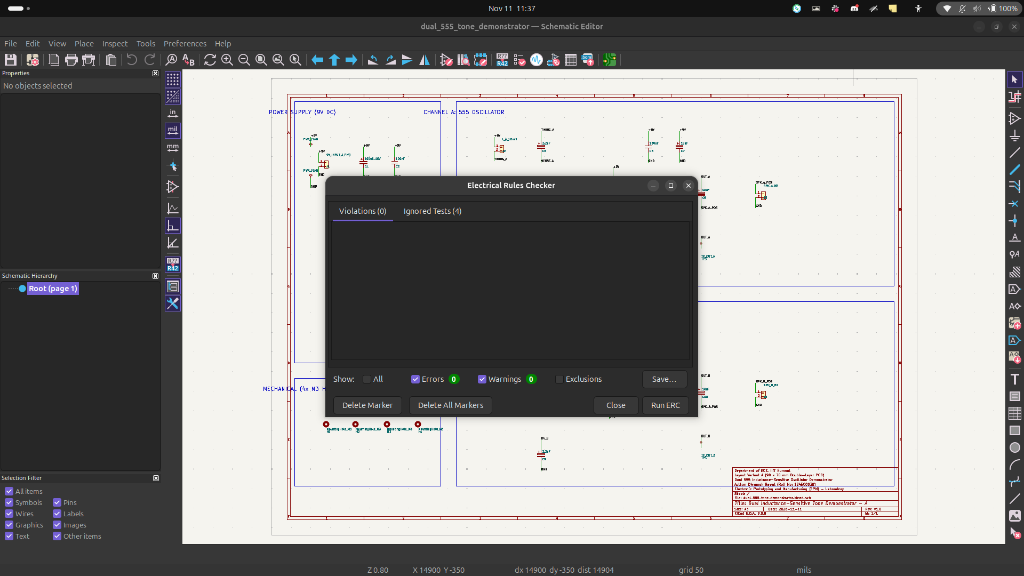
\includegraphics[width=0.98\textwidth]{screenshots/08_ERC_Verification_0_Errors.png}
    \caption{Uncropped screenshot of KiCad Electrical Rules Checker (ERC) dialog showing 0 errors and 0 warnings.}
\end{figure}

\vspace{-2mm}

\begin{table}[H]
\centering
\small
\renewcommand{\arraystretch}{1.2}
\begin{tabular}{|l|p{4.2cm}|l|p{4.2cm}|}
\hline
\textbf{ERC Result:} & 0 Errors, 0 Warnings (PASSED) & \textbf{KiCad Version:} & 9.0.8+dfsg-1 (Linux x86\_64) \\ \hline
\textbf{Schematic File:} & \texttt{dual\_555\_tone\_demonstrator.kicad\_sch} & \textbf{Sheet Name:} & Root Sheet (/) \\ \hline
\textbf{Power Drivers:} & \texttt{PWR\_FLAG} attached to +9V and GND & \textbf{Unconnected Pins:} & 0 Unintended Unconnected Pins \\ \hline
\end{tabular}
\end{table}

\clearpage

% =========================================================================
% PAGE 10: ITEM 9 - DESIGN RULES CHECK (DRC) SCREENSHOT
% =========================================================================
\section{Screenshot of Design Rules Check (DRC)}

Live KiCad PCB Editor Design Rules Checker dialog showing \textbf{0 Violations, 0 Unconnected Items, and 0 Schematic Parity Warnings}. Confirms 100\% routing completion, strict clearance compliance, zero courtyard overlaps, and full board-to-schematic netlist synchronization.

\vspace{3mm}

\begin{figure}[H]
    \centering
    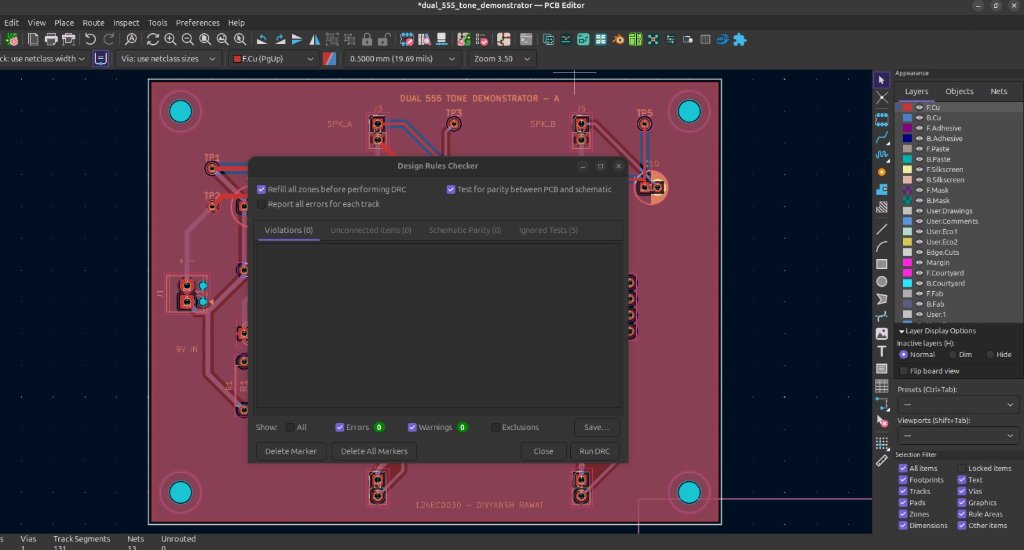
\includegraphics[width=0.98\textwidth]{screenshots/09_DRC_Verification_0_Violations.jpg}
    \caption{Uncropped screenshot of KiCad Design Rules Checker (DRC) dialog confirming 0 violations and 0 unconnected items.}
\end{figure}

\vspace{-2mm}

\begin{table}[H]
\centering
\small
\renewcommand{\arraystretch}{1.2}
\begin{tabular}{|l|p{4.2cm}|l|p{4.2cm}|}
\hline
\textbf{DRC Violations:} & 0 Violations & \textbf{Unconnected Items:} & 0 Unconnected Items \\ \hline
\textbf{Schematic Parity:} & 0 Parity Warnings (100\% Match) & \textbf{Overall DRC:} & 0 Errors, 0 Warnings \\ \hline
\textbf{Zone Refill Status:} & Zones Filled Prior to Check & \textbf{Board File:} & \texttt{dual\_555\_tone\_demonstrator.kicad\_pcb} \\ \hline
\end{tabular}
\end{table}

\clearpage

% =========================================================================
% PAGE 11: APPENDIX A - 3D MULTI-ANGLE VISUALIZATION
% =========================================================================
\appendix
\section{3D Multi-Angle Visualization Views}

Comprehensive 3D raytraced renders from four vantage points in KiCad 3D Viewer demonstrating component package fit, through-hole solder joints, connector orientations, and ground plane pours.

\vspace{3mm}

\begin{figure}[H]
    \centering
    \begin{subfigure}[b]{0.48\textwidth}
        \centering
        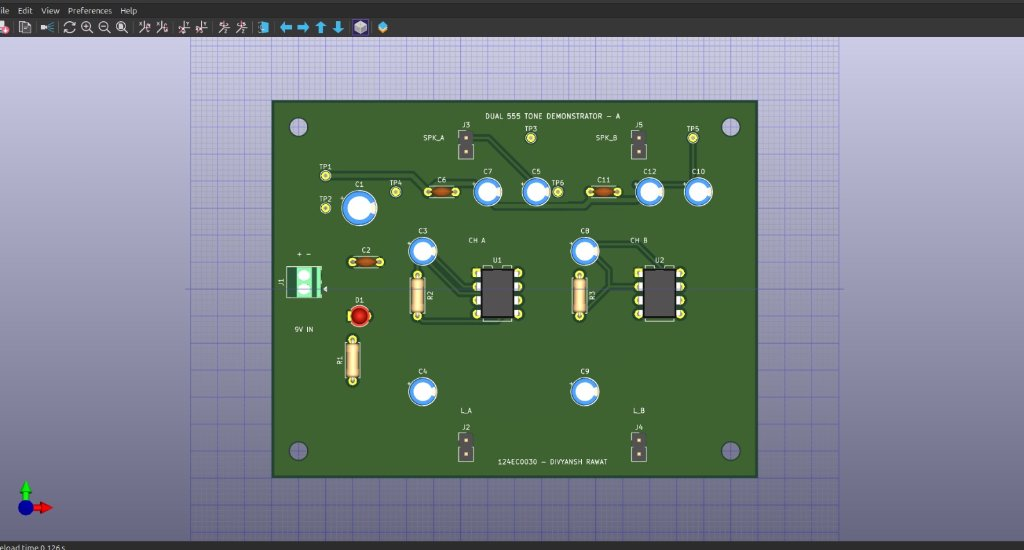
\includegraphics[width=\textwidth]{screenshots/3D_View_Top.jpg}
        \caption{Top Orthogonal View.}
    \end{subfigure}
    \hfill
    \begin{subfigure}[b]{0.48\textwidth}
        \centering
        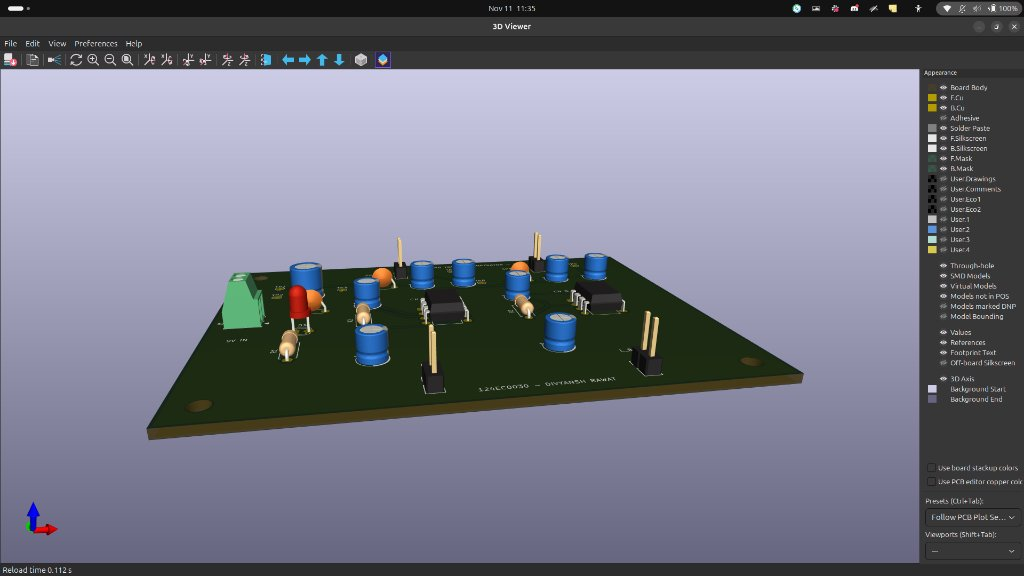
\includegraphics[width=\textwidth]{screenshots/3D_View_Isometric.jpg}
        \caption{Isometric Perspective View.}
    \end{subfigure}
    
    \vspace{4mm}
    
    \begin{subfigure}[b]{0.48\textwidth}
        \centering
        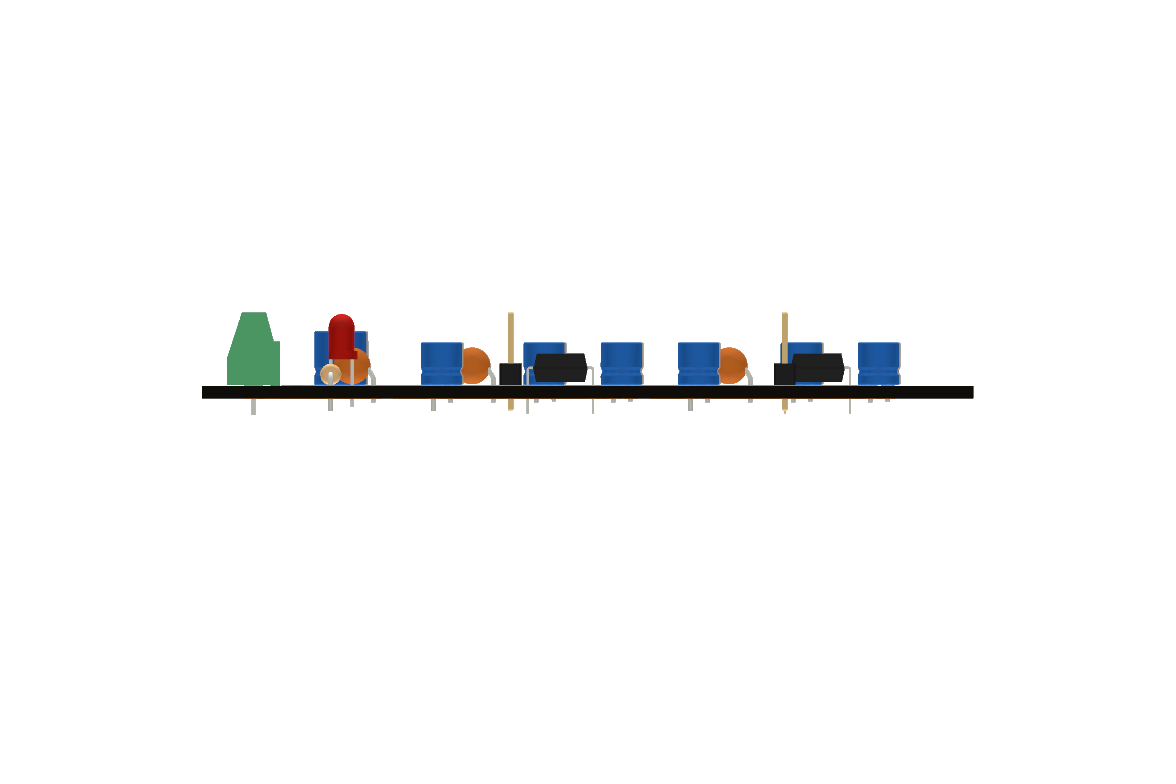
\includegraphics[width=\textwidth]{screenshots/3D_View_Front.png}
        \caption{Front Elevation View.}
    \end{subfigure}
    \hfill
    \begin{subfigure}[b]{0.48\textwidth}
        \centering
        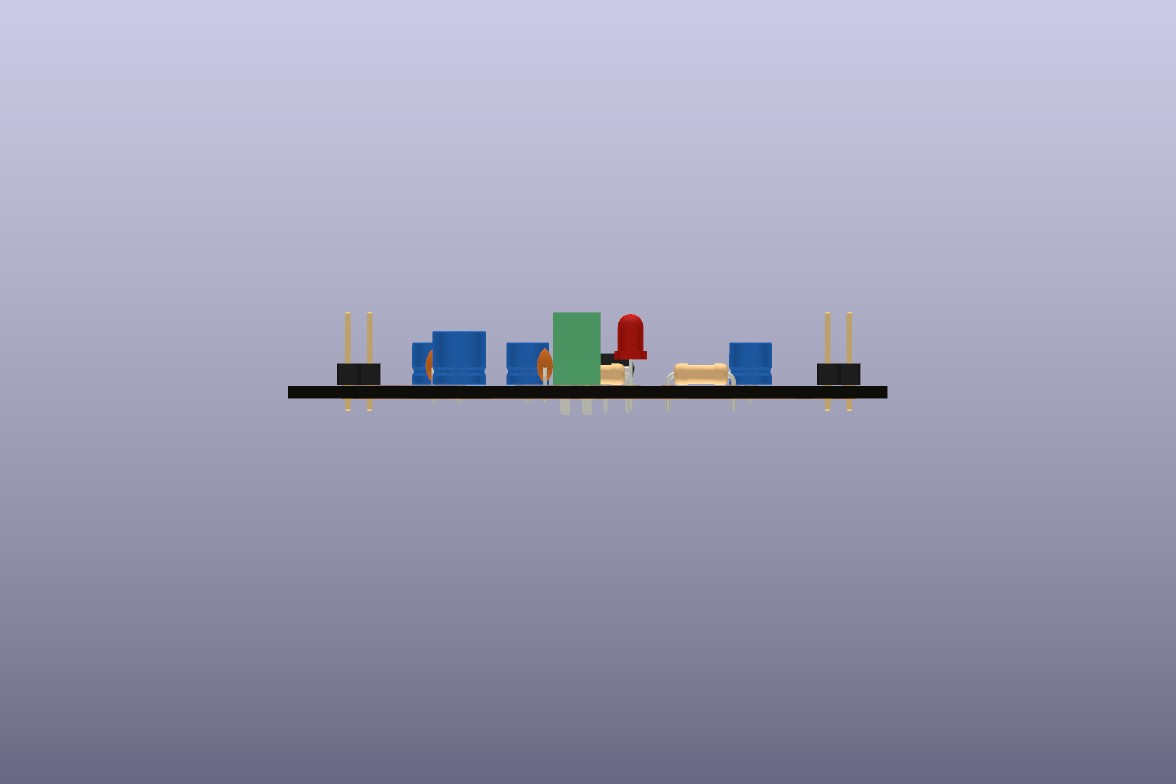
\includegraphics[width=\textwidth]{screenshots/3D_View_Side.jpg}
        \caption{Side Profile View.}
    \end{subfigure}
    \caption{Four-view 3D visualization gallery captured in KiCad 3D Viewer with realistic green soldermask.}
\end{figure}

\clearpage

% =========================================================================
% PAGE 12: APPENDIX B - BILL OF MATERIALS (BOM)
% =========================================================================
\section{Bill of Materials (BOM)}

Complete, verified Bill of Materials for the Dual Inductance-Sensitive Tone Demonstrator --- Layout Variant A ($90 \times 70$\,mm).

\vspace{3mm}

\begin{table}[H]
\centering
\small
\renewcommand{\arraystretch}{1.2}
\begin{tabularx}{\textwidth}{|c|>{\bfseries}p{2.2cm}|p{2.0cm}|p{4.2cm}|c|X|}
\hline
\textbf{\#} & \textbf{Ref} & \textbf{Value} & \textbf{Footprint} & \textbf{Qty} & \textbf{Description / Function} \\ \hline
1 & U1, U2 & NE555P & DIP-8\_W7.62mm & 2 & Precision Bipolar Timer IC \\ \hline
2 & J1 & 9V\_INPUT & TerminalBlock\_MPT-0.5-2\_P2.54mm & 1 & DC Power Input Terminal Block \\ \hline
3 & J2, J4 & L\_A, L\_B & PinHeader\_1x02\_P2.54mm\_Vertical & 2 & External Inductor (10\,mH) Connectors \\ \hline
4 & J3, J5 & SPK\_A, SPK\_B & PinHeader\_1x02\_P2.54mm\_Vertical & 2 & External Speaker ($8\,\Omega$) Connectors \\ \hline
5 & C1 & 100uF\_16V & CP\_Radial\_D6.3mm\_P2.50mm & 1 & Power Supply Bulk Reservoir Capacitor \\ \hline
6 & C2, C6, C11 & 100nF & C\_Disc\_D4.3mm\_W1.9mm\_P5.00mm & 3 & High-Frequency Ceramic Bypass Capacitors \\ \hline
7 & C3, C4, C8, C9 & 2.2uF\_16V & CP\_Radial\_D5.0mm\_P2.00mm & 4 & Astable Timing Electrolytic Capacitors \\ \hline
8 & C5, C7, C10, C12 & 10uF\_16V & CP\_Radial\_D5.0mm\_P2.00mm & 4 & AC Audio Output Coupling Capacitors \\ \hline
9 & R1 & 1k & R\_Axial\_DIN0207\_P7.62mm & 1 & Power LED Current-Limiting Resistor \\ \hline
10 & R2, R3 & 47k & R\_Axial\_DIN0207\_P7.62mm & 2 & Astable Timing Feedback Resistors \\ \hline
11 & D1 & PWR\_LED & LED\_D3.0mm & 1 & Green Power Status Indicator \\ \hline
12 & TP1--TP6 & TestPoint & TestPoint\_THTPad\_D1.5mm & 6 & Diagnostic Test Points (+9V, GND, Outs) \\ \hline
13 & H1--H4 & M3 Hole & MountingHole\_3.2mm\_M3 & 4 & M3 Mechanical Chassis Mounting Holes \\ \hline
\end{tabularx}
\end{table}

\end{document}
